\documentclass[10pt,twocolumn]{IEEEtran}

\usepackage{amsmath,amssymb}
\usepackage{graphicx}
\usepackage{booktabs}
\usepackage{url}
\usepackage{tikz}
\usetikzlibrary{arrows.meta,positioning}

\begin{document}

\title{Horizon Capital: A Multi-Agent Autonomous Trading System}

\author{Aaryan~Baadkar\\
\textit{Horizon Capital Project}\\
Email: aaryanbaadkar71@gmail.com}

\maketitle

\begin{abstract}
Claims about LLM-driven trading are easy to make and hard to check. Their
backtests are contaminated by survivorship bias and by selection on the data
used to report results, and the LLM's contribution is rarely separated from
the mechanical effect of trading differently. This paper is about the
checking.

\textbf{Horizon Capital} is an autonomous trading system organised as an
investment firm: strategy, portfolio, execution, risk, compliance, debate and
accounting agents under an executive AI CIO, coordinating over a
publish/subscribe bus. Signals come from rule-based sleeves; every mix change
had to clear gates fixed before evaluation on point-in-time data.
That discipline removed the project's motivating result, an edge that was
survivorship bias, and dropped a breadth-timing sleeve carrying
40\% of the mix once leave-one-out attribution showed the ensemble did better
without it. What survived compounds at 15.8\% on 2018--2024 and 13.0\% on an
untouched 2008--2017 holdout, against 13.6\% and 8.5\% for the S\&P~500, at
three-quarters of the index's volatility and a $-19.1\%$ drawdown where the
index lost $-51.9\%$. Deflating for twelve variants leaves the probability of
a positive true Sharpe at 0.72 and 0.85.

A pre-registered A/B experiment tested the component everyone assumes works. The debate gate ruled on 270 signals with the security's identity and
date withheld; binding it \emph{reduced} Sharpe from 0.89 to 0.81 while
deepening drawdown. A rate-matched control choosing at random scored 0.93, and
the panel beat only 5 of 25 such controls: the gate's apparent effect was a
fivefold drop in turnover, not judgment. It reverts to advisory-only; the
architecture contained the failure, a veto slot costing 0.08 of Sharpe rather
than a breached risk limit. The same protocol rejected a prediction-market
sleeve ($-8.1\%$), now disabled. A methodology that only ever approves is not
a methodology.
\end{abstract}

\begin{IEEEkeywords}
Multi-agent systems, large language models, algorithmic trading, momentum,
risk management, backtesting methodology, survivorship bias
\end{IEEEkeywords}

\section{Introduction}

Automated trading strategies are central to modern asset management, and a
growing literature applies deep reinforcement learning
\cite{yang2020ensemble,xiong2018practical,jiang2017deep,liu2020finrl} and, more
recently, large language models
\cite{yang2023fingpt,wu2023bloomberggpt,xiao2024tradingagents,yu2023finmem} to
the problem. Two gaps motivate this work.

First, \emph{architecture}. Most published systems collapse the investment
process into a single learned policy: one network observes prices and emits
orders. Real investment firms do not work this way. Signal generation,
position sizing, risk limits, compliance, execution, and accounting are
performed by different desks with different objectives and veto power over
one another. This separation is not bureaucratic overhead; it is the
mechanism by which firms prevent any single model's failure mode from
reaching the market unchecked.

Second, \emph{evaluation}. Backtests reported in the applied literature are
routinely contaminated by survivorship bias, lookahead in universe
construction, and post-hoc strategy selection \cite{bailey2014deflated,
lopezdeprado2018advances,harvey2016cross}. A strategy tuned until its
historical Sharpe ratio looks attractive has, in effect, been fit to the test
set. The problem is sharper for LLM-based signals, where the model's training
corpus may already contain the outcomes the backtest is trying to predict
\cite{glasserman2023lookahead}.

Horizon Capital addresses both gaps. It is a complete, runnable
system\footnote{Python 3.14, Rich terminal interface; local mode requires
only SQLite, no external services.} that models a hedge fund as an
organizational chart of decoupled agents coordinating over a
publish/subscribe message bus, with three nested gates between a strategy
signal and a broker order. Its signal layer is deliberately transparent,
built from rule-based momentum, trend, quality and regime primitives from the
empirical asset-pricing literature \cite{jegadeesh1993returns,faber2007tactical,
asness2019qmj}, while its \emph{judgment} layer uses multiple LLMs in an
adversarial debate protocol inspired by multi-agent deliberation
\cite{du2023improving,park2023generative}. Its evaluation discipline is
pre-registered: strategy changes must pass gates that are fixed \emph{before}
the candidate is evaluated, on point-in-time data the candidate never saw.

The contributions of this paper are:
\begin{enumerate}
\item A validation protocol for autonomous trading agents (point-in-time
universes, leave-one-out sleeve attribution, holdout gates fixed before
evaluation, and deflation for the number of variants tried), together with
a full account of what it rejected, this project's own first result included.
\item A pre-registered test of whether an LLM debate gate improves realized
outcomes, with two controls that this literature usually omits: prompts
blinded to the security's identity and date, and a gate that rejects at the
measured rate but chooses at random. The gate fails against the second
control, and that control is the point.
\item A firm-as-org-chart multi-agent architecture with a three-gate pipeline
(rule-based risk, LLM debate, execution guards) and per-asset-class broker
routing across equities, cryptocurrency and prediction markets.
\item Deployment lessons from live paper trading against a real brokerage
API, including a reconciliation guard pattern that generalizes to any system
whose local ledger can drift from broker state.
\end{enumerate}

The second contribution needs a boundary drawn around it. Nothing here shows
that LLMs cannot help a trading system. What it shows is that this gate, in
this configuration, on this signal stream, did not, and that without the
random-rejection control the opposite conclusion would have been reported,
because the gate did cut turnover fivefold and that alone moves the headline
numbers.

\section{Related Work}

\subsection{Reinforcement Learning for Trading}
Actor-critic methods (PPO, A2C, DDPG) have been applied to portfolio
trading, individually and as Sharpe-selected ensembles
\cite{yang2020ensemble,xiong2018practical,jiang2017deep}, packaged as
reusable libraries \cite{liu2020finrl}, and extended with graph
representations of inter-asset relations \cite{sun2024graphsage,
sun2024dynamic}, multi-asset agent hierarchies \cite{kim2025mama},
uncertainty-aware risk-sensitive networks \cite{park2024uncertainty}, and
multi-indicator state constructions \cite{liu2025qtmrl}. These systems learn
positions end-to-end from price features. Horizon Capital takes the opposite
position on interpretability, a concern the explainable-AI-in-finance
literature treats as a precondition for deployment rather than a nicety
\cite{cerneviciene2024xai,bartram2020ai}: positions come from transparent
rules whose historical behavior can be attributed sleeve by sleeve, and
learned components (LLMs) are confined to a veto role where their failure
mode is a rejected trade, not an unbounded position.

\subsection{LLMs and Agents in Finance}
Domain LLMs \cite{wu2023bloomberggpt,yang2023fingpt}, transformer sentiment
models applied to market text \cite{palomo2023tweet}, and machine-learned
manager selection \cite{ma2025hedge} have shown promise in signal extraction
and decision support. Closest to this work are LLM trading agents organised
as firms: TradingAgents assigns analyst, researcher and risk roles that argue
before a trade \cite{xiao2024tradingagents}, FinMem adds a layered memory and
character profile to a single agent \cite{yu2023finmem}, and QuantAgents
couples a multi-agent panel to simulated trading \cite{li2025quantagents}.
Multi-agent debate improves factuality and reasoning in general tasks
\cite{du2023improving}, and generative agent societies exhibit useful
division of labor \cite{park2023generative}. Horizon Capital applies both
ideas to trade approval specifically: debate with structured votes, role
rotation, and a consensus rule that fails \emph{closed} (no providers
$\Rightarrow$ reject) when the system trades autonomously. It differs
from the systems above in what it does with the result. The panel is treated
as a hypothesis to be tested against a rate-matched random control rather
than as a component whose value is assumed.

\subsection{Systematic Strategies and Validation}
The sleeves implement standard results: 12--1 cross-sectional and time-series
momentum \cite{jegadeesh1993returns,moskowitz2012tsmom}, the
10-month/200-day trend filter \cite{faber2007tactical}, quality-minus-junk
ranking \cite{asness2019qmj}, hierarchical risk parity
\cite{lopezdeprado2016hrp}, regime switching estimated from index returns
\cite{hamilton1989regime,kritzman2012regime}, and fractional-Kelly sizing
\cite{kelly1956,maclean2011kelly}. The evaluation discipline follows the
backtest-overfitting literature \cite{bailey2014deflated,
lopezdeprado2018advances,harvey2016cross}: deflated expectations, holdout
periods fixed in advance, and reporting of adverse results. Sampling error in
a Sharpe ratio estimated from one realized path \cite{lo2002statistics} and
survivorship and delisting bias in the universe
\cite{elton1996survivorship,shumway1997delisting} are treated as first-order
concerns rather than caveats, since both inflate exactly the statistic this
kind of system is judged on.

\section{System Architecture}

\subsection{Firm as an Organizational Chart}

Horizon Capital instantiates the departments of an investment firm as
independent asynchronous agents. Fig.~\ref{fig:pipeline} describes the
resulting trade pipeline. It shows the agents a trade intent passes through in
order (strategy, risk, portfolio with the debate panel attached to the
side, execution, broker), the message type carried on each edge, and the
three points at which the intent can be stopped: the rule-based risk check,
the LLM debate, and the execution-time guards. Nothing in the figure is a
direct function call; every edge is a message on the bus. The departments are:

\begin{itemize}
\item \textbf{Front office.} \emph{StrategyAgent} (signal generation from
the sleeve ensemble, Sec.~\ref{sec:sleeves}); \emph{PortfolioAgent}
(position sizing, NAV ownership, and the debate gate);
\emph{ExecutionAgent} (order routing and final guards); an investor-relations
agent (periodic reporting) and a sentiment agent (news-headline scoring).
\item \textbf{Middle office.} \emph{RiskAgent} (pre-trade limit checks and a
30-second VaR/CVaR/drawdown loop with a sticky kill switch);
\emph{ComplianceAgent} (restricted lists, concentration);
\emph{OperationsAgent} (stuck-order detection); \emph{DebateAgent}
(Sec.~\ref{sec:debate}); an alpha-decay monitor that watches for the concept
drift a static rule set cannot see \cite{wang2015concept}.
\item \textbf{Back office.} Accounting (P\&L, NAV reconciliation), IT
(process health, resource monitoring), and quantitative-data agents.
\item \textbf{Executive.} An AI Chief Investment Officer issuing periodic
strategic advisories, crisis responses to risk alerts, and (only under a
kill-switch state with high stated confidence) an override directive.
\end{itemize}

Agents never call one another directly. All coordination flows over a
namespaced publish/subscribe bus \cite{eugster2003faces}
(\texttt{horizon.\textit{area}.\textit{topic}})
with wildcard subscriptions; in local mode the bus is an in-process
asynchronous queue and all state persists to SQLite, so the entire firm runs
on a laptop with no external infrastructure. A supervisor restarts crashed
agents from heartbeats. This decoupling is what makes the gate structure
enforceable: the only path from a signal to an order is through messages
that the risk and debate agents can intercept.

\begin{figure}[t]
\centering
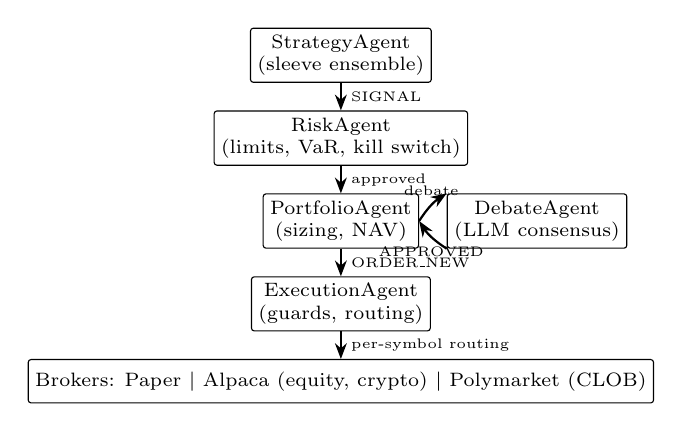
\begin{tikzpicture}[
  node distance=3.5mm and 3.5mm,
  box/.style={draw, rounded corners=1pt, align=center, font=\scriptsize,
              inner sep=2.5pt, minimum height=5.5mm},
  arr/.style={-{Stealth[length=2mm]}, thick}
]
\node[box] (strat) {StrategyAgent\\(sleeve ensemble)};
\node[box, below=of strat] (risk) {RiskAgent\\(limits, VaR, kill switch)};
\node[box, below=of risk] (port) {PortfolioAgent\\(sizing, NAV)};
\node[box, right=of port] (debate) {DebateAgent\\(LLM consensus)};
\node[box, below=of port] (exec) {ExecutionAgent\\(guards, routing)};
\node[box, below=of exec] (brokers) {Brokers: Paper $|$ Alpaca (equity, crypto) $|$ Polymarket (CLOB)};
\draw[arr] (strat) -- node[right, font=\tiny]{SIGNAL} (risk);
\draw[arr] (risk) -- node[right, font=\tiny]{approved} (port);
\draw[arr] (port.east) to[bend left=12] node[above, font=\tiny]{debate} (debate.north west);
\draw[arr] (debate.south west) to[bend left=12] node[below, font=\tiny]{APPROVED} (port.east);
\draw[arr] (port) -- node[right, font=\tiny]{ORDER\_NEW} (exec);
\draw[arr] (exec) -- node[right, font=\tiny]{per-symbol routing} (brokers);
\end{tikzpicture}
\caption{The trade pipeline. Three nested gates separate a strategy signal
from a broker order: rule-based risk checks, the LLM debate (binding in
fully-autonomous mode), and execution-time guards.}
\label{fig:pipeline}
\end{figure}

\subsection{Trade Pipeline and Operating Modes}

A trade intent traverses the path in \eqref{eq:pipeline}:
\begin{equation}
\label{eq:pipeline}
\begin{aligned}
\text{Strategy} \;\xrightarrow{\;\textsc{signal}\;}\; &\text{Risk}
  \;\rightarrow\; \text{Portfolio} \;(+\,\text{Debate})\\
  &\rightarrow\; \text{Execution} \;\rightarrow\; \text{Broker}.
\end{aligned}
\end{equation}
Equation~(\ref{eq:pipeline}) states the only route from a strategy signal to a
broker order, and it is a total ordering rather than a summary: each arrow is a
message on the bus, each stage can terminate the intent, and there is no edge
that skips a stage. The debate panel is written in parentheses because it is
consulted by the PortfolioAgent rather than being a stage of its own, which is
why disabling it (Sec.~\ref{sec:abresults}) leaves the remaining path
unchanged.

The RiskAgent enforces per-position weight caps (20\% of NAV) and daily-loss
limits symbol-agnostically. The PortfolioAgent, sole owner of NAV, sizes
approved signals against database-backed cash balances (the key-value cache
is a mirror, never the source of truth). The ExecutionAgent applies final
guards: kill-switch state, cash sufficiency, and a naked-short prohibition,
then routes per symbol (equities and cryptocurrency to a paper simulator
or the Alpaca API, prediction-market symbols to a Polymarket CLOB client),
so no order can reach a broker that does not trade its asset class.

Three operating modes trade off autonomy against oversight:
\emph{paper-trading} (immediate simulated execution),
\emph{human-approval} (orders queue for interactive approve/reject), and
\emph{fully-autonomous}, in which the debate gate is binding and, absent any
LLM provider, fails closed by rejecting the signal.

\subsection{Execution Realism}
The paper broker charges commissions on every fill and applies an
Almgren--Chriss-style \cite{almgren2001optimal} temporary-impact model, so
simulated fills degrade with participation. Realized P\&L is
commission-inclusive by construction (commissions hit realized P\&L on every
fill, including opening legs), which forces cash and P\&L ledgers to agree
exactly, a property the test suite verifies.

\section{Strategy Layer: Validated Sleeve Ensemble}
\label{sec:sleeves}

Signals come from independent \emph{sleeves}, each a pure function from
historical bars to target portfolio weights, combined by fixed mix weights.
The production mix (Sec.~\ref{sec:eval}) is:

\begin{itemize}
\item \textbf{Research stack} (weight 0.500, weekly). A Gaussian-mixture
regime model \cite{kritzman2012regime} on index returns gates the book:
in \textsc{risk-off} regimes capital moves to an inverse-volatility blend of
long-duration Treasuries and gold; in \textsc{risk-on} regimes the sleeve
ranks the point-in-time S\&P~500 universe by 12--1 time-series momentum
\cite{jegadeesh1993returns} and quality \cite{asness2019qmj}, takes the top
five names, weights them by hierarchical risk parity
\cite{lopezdeprado2016hrp} (chosen over mean-variance optimization
\cite{markowitz1952} because the latter's weights are notoriously sensitive to
estimation error in the covariance matrix at this universe size), and caps
each weight at half-Kelly
\cite{kelly1956}.
\item \textbf{Trend filter} (0.333, weekly). Faber's 200-day moving-average
rule \cite{faber2007tactical} on the index proxy (long above trend, cash
below), with a realized-volatility cap.
\item \textbf{Momentum rank} (0.167, monthly). Cross-sectional 12--1
momentum, top three names, equal weight. The live 20\% position cap contains
its standalone drawdown (max $-25.4\%$ capped, versus $-59.5\%$ uncapped in
an unconstrained harness).
\end{itemize}

The StrategyAgent aggregates sleeve targets and emits a signal only when a
symbol's net target drifts more than 50 basis points, keeping turnover low.

\textbf{Optional, unvalidated sleeves} for cryptocurrency (a Faber-style
200-day trend rule on BTC and ETH with an annualized-volatility damper) and
prediction markets (Sec.~\ref{sec:polymarket}) are carved out of the mix
pro-rata \emph{only when explicitly enabled}, a construction that leaves the
validated equity mix byte-identical when they are off, a property pinned
by a regression test. Both default to off; the prediction-market sleeve
remains off because it failed its gate.

\section{The LLM Debate Gate}
\label{sec:debate}

In fully-autonomous mode every sized trade must survive a structured debate
among four adversarial analyst roles: \textsc{strategy} (bull case),
\textsc{risk} (bear case), \textsc{sentiment} (news and crowd positioning),
and \textsc{portfolio} (fit with existing exposure). Each debater receives
the same grounded context (signal metadata, market regime, cached sentiment,
portfolio risk metrics) with explicit instructions to reason only from the
data provided, and returns a free-text \texttt{argument} together with the
structured verdict of \eqref{eq:vote}:
\begin{equation}
\label{eq:vote}
\begin{aligned}
\texttt{vote} \;&\in\; \{\textsc{for},\ \textsc{against},\ \textsc{abstain}\},\\
\texttt{confidence} \;&\in\; [0,1].
\end{aligned}
\end{equation}
Equation~(\ref{eq:vote}) states the contract the consensus rule depends on: a
debater's opinion reaches the tally only as a discrete vote paired with a
scalar confidence, and \textsc{abstain} is a first-class option rather than a
missing value. Free text is logged for audit but never parsed for intent, so a
debater that argues persuasively and votes \textsc{against} counts as against.

\textbf{Provider diversity.} Roles are assigned round-robin (or pinned by
configuration) across the available LLM providers, so different model
families argue different perspectives. This is a property of the
implementation, not of the experiment reported in Sec.~\ref{sec:aitest}: that
run had one provider available and therefore exercised role diversity without
model-family diversity. It is flagged here rather than left for the
architecture description to imply otherwise.

\textbf{Perspective rotation.} In round two each debater is reassigned the
\emph{opposite} role (bull argues the bear case, sentiment argues portfolio
fit) with the round-one transcript in context, and must engage the strongest
opposing argument. This forces genuine consideration of counterarguments
and measurably reduces same-model agreement bias \cite{du2023improving}.

\textbf{Consensus.} With $F$, $A$ the \textsc{for} and \textsc{against} vote
sets over both rounds and $c_i$ the vote confidences, the trade is approved iff
both conditions of \eqref{eq:consensus} hold:
\begin{equation}
\label{eq:consensus}
\begin{aligned}
\frac{\sum_{i \in F} c_i}{\sum_{i \in F \cup A} c_i} \;&>\; 0.55,\\[2pt]
\frac{|F|}{|F| + |A|} \;&\geq\; 0.6,
\end{aligned}
\end{equation}
Equation~(\ref{eq:consensus}) states that approval requires a supermajority on
two independent counts: the first line is the confidence-weighted \textsc{for}
share, which lets a strongly held minority view block a lukewarm majority, and
the second is the raw head-count share, which stops a single high-confidence
debater from carrying the vote alone. Both denominators exclude abstentions, so
abstaining shrinks the panel rather than voting with either side, which is why
the structurally abstaining \textsc{sentiment} role (Sec.~\ref{sec:limits})
lowers effective panel size instead of biasing the verdict. Malformed model
output
degrades to \textsc{abstain} rather than being reprompted, and if no
provider is available the debate \emph{rejects}: in autonomous mode the
system never trades on the absence of judgment. All arguments, votes, and
conclusions persist to an auditable session log.

\section{Validation Methodology}
\label{sec:method}

Three rules govern every strategy change.

\subsubsection{Point-in-time universes} Ranking today's index constituents
backward in time implicitly conditions on survival, a bias with a long
measured history in fund and security samples alike
\cite{elton1996survivorship,shumway1997delisting}. The first backtests in this
project made exactly that error, and the apparent edge, which motivated the
project, disappeared under a reconstructed point-in-time S\&P~500
membership series. That is reported here as a headline result rather than an
embarrassment: the pipeline that revealed it is the product.

\subsubsection{Leave-one-out attribution} Each sleeve is removed from the
mix in turn and the ensemble re-evaluated on PIT data; a sleeve earns its
weight only if removing it hurts. This is how a breadth-timing sleeve,
attractive standalone and previously 40\% of the mix, was found to drag
the ensemble (Sec.~\ref{sec:eval}) and dropped.

\subsubsection{Pre-registered holdout gates} Candidate mixes are selected on
one PIT period (2018--2024) and must then pass acceptance criteria,
fixed \emph{before} evaluation, on an unseen holdout (2008--2017)
spanning the global financial crisis: Sharpe not worse than the incumbent,
maximum drawdown not deeper, comparable CAGR. Candidates that fail ship
disabled, with the adverse result recorded. No signal parameter is tuned on
holdout data.

\section{Performance Evaluation}
\label{sec:eval}

All figures below were regenerated from the repository's validation
harnesses immediately before submission of this draft (yfinance daily bars;
identical fill model across all arms; delisted-symbol coverage gaps noted
in Sec.~\ref{sec:limits} bias all arms equally).

\subsection{Benchmark Selection}
\label{sec:benchmarks}

Comparing a hedge-fund system only against a long-only equity index is a weak
test: the index is not a peer. Three benchmarks are therefore reported on every
window, computed from the same daily bars, the same metric definitions and the
same risk-free series as every strategy row.

That series deserves a note, because an earlier draft of this work got it
wrong: it charged a flat 4\% risk-free rate on both windows. The realized
13-week Treasury bill averaged 0.31\% over 2008--2017 (below 1\% on 88\% of
trading days) and 2.33\% over 2018--2024. A fixed hurdle is not a
conservative simplification here: it is biased between arms, because the same
absolute hurdle is a larger fraction of a smaller volatility denominator and
therefore penalises a low-volatility strategy more than a high-volatility
benchmark. Every ratio in this paper is now computed against the realized daily
bill rate, applied identically to strategy and benchmark rows. The correction
raises every row; it does not change the ordering of any of them. Sharpe ratios
throughout are the annualized mean of daily excess return over its annualized
standard deviation \cite{sharpe1994}, and its sampling error on a single path
is not negligible \cite{lo2002statistics}. \textbf{SPY} is the S\&P~500
buy-and-hold reference. \textbf{QAI} (IQ Hedge Multi-Strategy Tracker) is an
investable replication of the aggregate hedge-fund industry return stream and
stands in for the licensed HFRI-type ``industry average'' indices; notably, a
replication ETF is free of the survivorship and backfill bias documented in
self-reported hedge-fund indices \cite{fung2000performance}, so if anything it
is the stricter comparison. \textbf{AOR} (iShares Core Growth Allocation) is a
conventional 60/40 balanced portfolio, the default alternative use of the
capital. Both peer funds post-date the start of the 2008--2017 holdout and
therefore skip part of the crisis; each one's realized coverage is reported
rather than silently spliced, and the relative drawdown advantage on that
window should be read as a lower bound. The industry proxy is the row the
risk-free correction moves most, since a fixed hurdle bears hardest on the
vehicle with the least volatility to spread it over: its selection-period
Sharpe rises from $-0.21$ under the old flat rate to $0.05$ under the realized
one. The corrected figure is reported even though it narrows the lead claimed
here, because it is the right one.

\subsection{Results on Both Windows}

Table~\ref{tab:perf} reports every arm on both windows under one harness, one
fill model and one risk-free series. The pattern is the same in each: the mix
earns more than the index while taking materially less risk, and the advantage
comes from what it does in bad markets rather than good ones.

On the 2018--2024 selection period the mix compounds at 15.8\% against the
index's 13.6\%, at three-quarters of its volatility and roughly half its
maximum drawdown, while holding an average gross exposure of only 78\%: it
outperforms with a standing cash buffer. On the 2008--2017 holdout, which the
candidate had never seen, the gap widens: 13.0\% against 8.5\%, and a maximum
drawdown of $-19.1\%$ where the index lost $-51.9\%$. A \$100{,}000 account
would have finished that decade at \$340{,}322 against the index's \$226{,}948,
and would have spent 360 trading days below a prior peak rather than 835.

The down-capture column is the clearest statement of where the edge lives. On
the holdout the mix captured 47\% of the index's down-day moves; through the
worst equity market since 1929 it took under half the damage. That is also why
Sortino (1.35) exceeds Sharpe (0.99) by a wide margin: the volatility the
strategy does carry is disproportionately upside, and a denominator that
counts only downside deviation \cite{sortino1994downside} rewards it
accordingly. Calmar \cite{young1991calmar} tells the same story more bluntly:
0.68 against the index's 0.16, a four-fold advantage in return earned per
unit of drawdown suffered.

Against the peer benchmarks the mix leads on return and on every risk-adjusted
measure in both windows. The hedge-fund industry proxy is the instructive
comparison rather than the flattering one: it runs at a third of the mix's
volatility and, on the holdout, a much shallower drawdown, because it is built
to a different mandate. It also compounds at 3.1\% against the mix's 13.0\%.
Its down-capture of 25\% is genuinely better; its Calmar of 0.41 is not,
because the protection is paid for in return.

Fig.~\ref{fig:equity} describes the same comparison as a path rather than a
table. It plots the mix and the index, each indexed to 100 at the start of the
window it belongs to, with the selection period in the upper
panel and the holdout in the lower one. The two curves say something the
summary statistics cannot: the mix does not win by rising faster in good years
(through 2019 and 2021 the index tracks it closely) but by declining less
in 2020, 2022 and above all 2008--2009, where the index halves and the mix does
not. The separation in each panel opens at a drawdown and is never given back.

\begin{table*}[t]
\caption{Performance on both evaluation windows. Identical harness, fill model
and risk-free series across every row. Sortino replaces total volatility with
downside deviation; Calmar is CAGR over maximum drawdown; down-capture is the
strategy's mean return on days the index fell, as a percentage of the index's;
lower is better. Final value is from \$100{,}000 invested at the window
start. $^\dagger$QAI and AOR post-date the start of the holdout (88\% and 91\%
coverage) and therefore miss part of the 2008 crash, which flatters their
drawdown figures.}
\label{tab:perf}
\centering
\begin{tabular}{lcccccccr}
\toprule
Variant & CAGR & Vol. & Sharpe & Sortino & Calmar & MaxDD & Down-cap. & Final \\
\midrule
\multicolumn{9}{l}{\emph{Selection period, PIT 2018--2024}} \\
Production mix & \textbf{15.8\%} & 15.3\% & \textbf{0.89} & \textbf{1.16} & \textbf{0.88} & $\mathbf{-18.0\%}$ & \textbf{63\%} & \textbf{\$278{,}355} \\
Prior mix (w/ breadth) & 14.6\% & 16.0\% & 0.79 & 1.03 & 0.60 & $-24.2\%$ & 72\% & \$259{,}383 \\
SPY buy-and-hold & 13.6\% & 19.5\% & 0.64 & 0.78 & 0.40 & $-33.7\%$ & n/a & \$244{,}206 \\
Hedge-fund industry (QAI) & 2.5\% & 6.4\% & 0.05 & 0.07 & 0.16 & $-14.9\%$ & 28\% & \$118{,}499 \\
60/40 balanced (AOR) & 5.9\% & 11.5\% & 0.36 & 0.45 & 0.26 & $-22.9\%$ & 58\% & \$149{,}254 \\
\midrule
\multicolumn{9}{l}{\emph{Holdout period, PIT 2008--2017 (unseen at selection)}} \\
Candidate (production) & \textbf{13.0\%} & 12.9\% & \textbf{0.99} & \textbf{1.35} & \textbf{0.68} & $\mathbf{-19.1\%}$ & \textbf{47\%} & \textbf{\$340{,}322} \\
Incumbent (w/ breadth) & 13.0\% & 14.8\% & 0.88 & 1.18 & 0.48 & $-26.9\%$ & 67\% & \$337{,}758 \\
SPY buy-and-hold & 8.5\% & 20.3\% & 0.49 & 0.60 & 0.16 & $-51.9\%$ & n/a & \$226{,}948 \\
Hedge-fund industry (QAI)$^\dagger$ & 3.1\% & 6.0\% & 0.51 & 0.63 & 0.41 & $-7.7\%$ & 25\% & \$130{,}768 \\
60/40 balanced (AOR)$^\dagger$ & 10.2\% & 13.6\% & 0.77 & 0.90 & 0.42 & $-24.4\%$ & 61\% & \$242{,}028 \\
\bottomrule
\end{tabular}
\end{table*}

\begin{figure}[t]
\centering
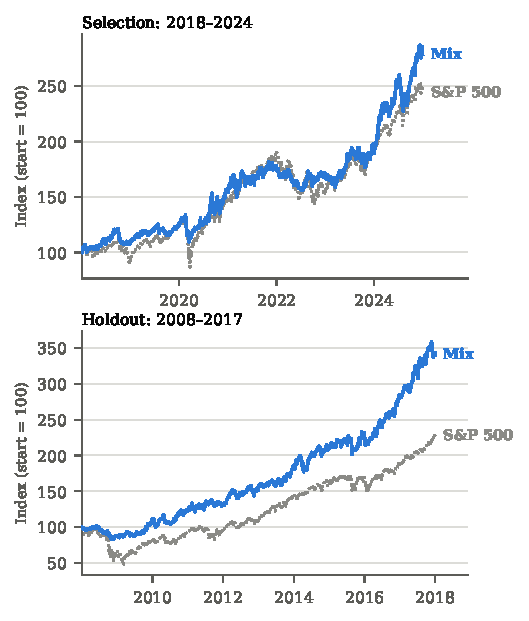
\includegraphics[width=\columnwidth]{fig_equity.pdf}
\caption{Production mix against the S\&P~500, both evaluation windows, each
normalized to 100 at the window start. The mix is not merely higher: it is
flatter through the drawdowns that matter: the 2020 crash and the 2022
decline in the upper panel, and the 2008--2009 crisis in the lower one, where
the benchmark loses roughly half its value and the mix does not. Series differ
in dash pattern as well as color so the figure survives grayscale printing.}
\label{fig:equity}
\end{figure}

\subsection{Sleeve Attribution}

Table~\ref{tab:loo} decomposes the ensemble. Each sleeve is shown standalone
and via leave-one-out (LOO): the mix re-run with that sleeve removed and
weights renormalized. Under the pre-registered rule (LOO is decisive, not
standalone performance), a sleeve whose removal \emph{raises} mix Sharpe
drags, and the breadth sleeve raised it from 0.79 to 0.89. It had carried 40\%
of the weight. It was dropped.

The rest of the decomposition is why the ensemble is an ensemble rather than a
single sleeve. The research stack is load-bearing: removing it costs 0.17 of
Sharpe, more than any other sleeve contributes. The trend filter is the
interesting case. Standalone it is the worst sleeve in the book, with a Sharpe
of $-0.05$: it spends most of its life in cash and earns almost nothing.
Removing it costs 0.03. It is carried not for return but for what it does to
the shape of the drawdown, with a solo maximum drawdown of $-4.0\%$ against
the ensemble's $-18.0\%$, and dropping it would be a decision to accept a
worse crisis in exchange for a rounding error of Sharpe. Momentum rank carries
0.05. Standalone daily-return correlations between the sleeves range
0.40--0.63, which is the diversification the construction is buying.

A top-10 variant of momentum rank was evaluated separately under the same rule
and \emph{failed} its gate; top-3 was retained.

\begin{table}[t]
\caption{Per-sleeve attribution, PIT 2018--2024. LOO = mix re-run without
that sleeve (weights renormalized). Full-mix Sharpe = 0.79. Recomputed against
the realized risk-free series; all four verdicts are unchanged from the
flat-rate computation under which the drop decision was originally made.}
\label{tab:loo}
\centering
\begin{tabular}{lcccc}
\toprule
& \multicolumn{2}{c}{Standalone} & \multicolumn{2}{c}{Leave-one-out} \\
Sleeve & Sharpe & MaxDD & Sharpe & Verdict \\
\midrule
Breadth-timing & 0.44 & $-35.2\%$ & \textbf{0.89} & drags (dropped) \\
Research stack & 0.72 & $-16.4\%$ & 0.63 & carries \\
Trend filter & $-0.05$ & $-4.0\%$ & 0.76 & neutral/hedge \\
Momentum rank & 0.70 & $-25.4\%$ & 0.74 & carries \\
\bottomrule
\end{tabular}
\end{table}

\subsection{Pre-Registered Holdout Gate}

The holdout rows of Table~\ref{tab:perf} are also an acceptance test. Two gates
were fixed before the candidate was evaluated on 2008--2017: G1, candidate
Sharpe strictly above the incumbent's; G2, maximum drawdown no more than five
points deeper. Both passed, and not narrowly: Sharpe 0.99 against 0.88, and a
drawdown 7.8 points \emph{shallower} rather than deeper. The candidate reaches
the same 13.0\% CAGR as the incumbent on lower volatility (12.9\% vs.\ 14.8\%)
and lower gross exposure (75\% vs.\ 94\%): the same return from a smaller,
calmer book.

The holdout matters more than the selection period, for two reasons. It was
never used to choose anything, and it contains the only genuine stress test
available in recent history. A strategy whose drawdown discipline is real
should show it there, and this one does: $-19.1\%$ against the index's
$-51.9\%$, with 47\% down-capture.

\subsection{Correcting for Multiple Testing}
\label{sec:dsr}

A Sharpe ratio selected as the best of several trials is biased upward, and
Sec.~\ref{sec:method} concedes that several sleeve mixes were evaluated. Raw
Sharpe ratios therefore overstate the evidence and are deflated here
(Table~\ref{tab:dsr}). The probabilistic Sharpe ratio (PSR) gives the
probability that the \emph{true} Sharpe exceeds a benchmark after correcting
for the skew and excess kurtosis of the realized return distribution
\cite{bailey2012psr}; the deflated Sharpe ratio (DSR) additionally discounts
for having chosen the best of $N$ trials \cite{bailey2014deflated}, the same
multiple-testing problem that inflates published factor discoveries
\cite{harvey2016cross}.

Rather than assume a flattering trial count, the deflation uses the twelve
Sharpe ratios this project actually produced (the full mix, four standalone
sleeves, four leave-one-out mixes, the rejected momentum top-10 variant, and
the holdout incumbent/candidate pair), whose observed spread ($-0.72$ to
$0.77$, variance $0.159$) is wide, and a wide spread deflates harder than a
generic assumption would.

The edge survives on both windows, more comfortably on the one that matters.
The probability that the true Sharpe is positive is 0.99 on the selection
period and 0.999 on the holdout; that it beats the index's is 0.74 and 0.94;
and after deflating for the search, 0.72 and 0.85 (Table~\ref{tab:dsr}). The
holdout is stronger on every measure, which is the right way round: it is the
period that was not selected on. The inference stops there: a 0.74
probability of beating the index on the selection window is evidence, not
proof, and is exactly the kind of number an undeflated Sharpe ratio would have
disguised.

\begin{table}[t]
\caption{Probabilistic and deflated Sharpe ratios for the production mix,
computed against the realized risk-free series. PSR corrects for the skew and
excess kurtosis of the return distribution; DSR additionally deflates for
selection across the 12 strategy variants this project evaluated.}
\label{tab:dsr}
\centering
\begin{tabular}{lccccc}
\toprule
Window & Days & SR & PSR$>$0 & PSR$>$SPY & DSR \\
\midrule
Selection 2018--2024 & 1{,}760 & 0.89 & 0.990 & 0.742 & 0.719 \\
Holdout 2008--2017 & 2{,}517 & 0.99 & 0.999 & 0.941 & 0.846 \\
\bottomrule
\end{tabular}
\end{table}

\subsection{An Adverse Result: Prediction-Market Momentum}
\label{sec:polymarket}

The system ingests Polymarket prediction-market prices (Gamma metadata,
CLOB midpoints) as first-class symbols with real execution support. Prediction
markets aggregate dispersed information into a price
\cite{wolfers2004prediction}, which motivated the hypothesis that event
probabilities drift (informed flow moves prices before resolution), and a
7-day probability-momentum sleeve was built to exploit it (long markets whose
YES price rose $\geq 5$ percentage points, mid-price restricted to
$[0.10, 0.90]$ to avoid resolution tails, 25\% per-market cap). Replayed
day-by-day over CLOB price history for the highest-volume markets
(Table~\ref{tab:pm}), the sleeve \emph{lost} money. Under the gate protocol
of Sec.~\ref{sec:method} it therefore ships disabled. The result is reported
at equal prominence with the positive ones; a validation methodology that
only ever approves is not a methodology.

\begin{table}[t]
\caption{Prediction-market momentum sleeve backtest (CLOB daily history,
highest-volume markets, 365-day window). Gate: \textbf{failed}; sleeve
ships disabled.}
\label{tab:pm}
\centering
\begin{tabular}{lc}
\toprule
Metric & Value \\
\midrule
Markets traded & 3 of 5 discovered \\
Aggregate total return & $-8.1\%$ \\
Sharpe ratio & $-0.18$ \\
Max drawdown & $-22.8\%$ \\
Daily hit rate & 43.3\% \\
\bottomrule
\end{tabular}
\end{table}

The caveats attached to this backtest apply to most published
prediction-market results: short history, volume-skewed market selection,
no order-book depth in fills, and binary-resolution jump risk that daily
bars understate.

\subsection{Live Deployment: the Reconciliation Guard}
\label{sec:live}

The full pipeline has run live against the Alpaca paper-trading API:
sleeve signals produced real API orders, polled to terminal fills
(fractional shares included), with cash settled atomically exactly once per
order. The launch surfaced a failure mode that appears underreported, though
its consequences in production systems are not \cite{sec2013knight,
kirilenko2017flash}. The
local ledger was initialized with \$1M while the brokerage account held
\$100k of paper equity; sizing against local NAV therefore produced
$3.5\times$ accidental margin exposure at the broker. The fix is a
\emph{startup reconciliation guard}: on connect, the system compares
broker equity to local NAV, reports position diffs, and, on a mismatch
exceeding 2\%, raises a critical alert and falls back to simulated
execution rather than trading a ledger it cannot trust. In subsequent runs
the guard fired correctly and refused live routing until the accounts were
re-synchronized. Any architecture whose internal state can drift from
broker truth needs an equivalent gate.

\subsection{Operational Robustness}

The firm survives its own components failing: a supervisor restarts crashed
agents from missed heartbeats (exercised in a boot-time database-contention
incident that crashed four agents; all recovered without operator action,
and the root cause was subsequently fixed), a sticky kill switch halts
trading on drawdown breaches until a human clears it, and alerts route to
console, Telegram, and e-mail. A template-based trade journal narrates every
fill, kill-switch event, and debate conclusion to a daily Markdown file
independent of any LLM. The codebase carries 467 automated tests, including
regression pins on the validated mix weights and on cash/P\&L consistency.

\section{Isolating the Debate Gate}
\label{sec:aitest}

The results above isolate the rule-based signal layer. What they do not
measure is the marginal contribution of the LLM debate gate itself. This
section reports that experiment.

\textbf{Design.} Two arms consume an \emph{identical} signal stream under an
identical fill model: (A) debate gate disabled, so every risk-approved signal
executes; (B) debate gate binding, so a signal executes only on an
\textsc{approved} conclusion from the multi-model debate of
Sec.~\ref{sec:debate}, and a rejected signal leaves that symbol at its
previous target weight, so the gate vetoes entries and exits alike. Sizing,
risk limits and execution are shared, so divergence is attributable to the
gate alone. Sleeve targets are a pure function of bars and date rather than of
the portfolio, which is what allows both arms to consume a byte-identical
signal stream even after their holdings diverge.

\textbf{Replay rather than forward test.} The pre-registered metrics include
Sharpe, maximum drawdown and turnover, which require hundreds of trades; live
paper trading emits a handful per week. The experiment therefore replays the
production mix over the 2018--2024 PIT window and routes every signal the live
StrategyAgent would have emitted (the same 50~bp drift rule) through the real
debate engine.
As a pre-registered validity check, arm~A must reproduce the published
production mix of Table~\ref{tab:perf} within $\pm 0.02$ Sharpe before any LLM
is called; it does (0.89 against 0.89, maximum drawdown $-18.0\%$ in both),
which
establishes that the replayed system is the published one.

\textbf{Hindsight leakage, measured rather than assumed away.} An LLM trained
on data after the evaluation window may recall what a given stock did, and the
effect is large enough to have been measured directly in GPT-based return
prediction \cite{glasserman2023lookahead}. The
primary arm therefore \emph{blinds} the panel: the prompt carries no ticker, no
date and no price level, only scale-free features (cross-sectional momentum
percentile, distance from the 200-day average, realized volatility, drawdown
from the 52-week high, correlation to the index, and the regime label). A
debater sees ``\textsc{asset} (identity withheld)'' and six numbers that
describe thousands of (security, date) pairs, so there is no key with which to
retrieve an outcome. A secondary \emph{unblinded} arm restores the ticker and
the as-of date on the same signals; the paired difference in verdicts is the
estimate of exploitable leakage, and is reported in
Table~\ref{tab:leak}.

\textbf{Deployed configuration.} The live DebateAgent does not debate every
signal: a cost gate spends a bounded daily budget on the strongest signals and
releases the remainder un-debated. Arm~B reproduces that behaviour (the
strongest signals are judged by the panel and the rest trade on the quant
signal), so the measured effect is the effect on the system as deployed
rather than on a hypothetical one that debates everything. The coverage
achieved is reported with the result.

\textbf{Arm C: a rate-matched random gate.} A gate that vetoes a large share of
trades mechanically reduces exposure and turnover, and in a trending sample
that alone can move the Sharpe ratio. ``Arm~B beat arm~A'' would therefore not
establish that the panel chose \emph{well}, only that it traded \emph{less}.
Arm~C is a control that holds the rejection rate at arm~B's measured value
while destroying the choice, accepting at random; twenty-five such gates give a
null distribution. Arm~B counts as evidence of judgment only if it clears that
distribution.

\textbf{Pre-registered metrics.} (i) approval/rejection/abstention rates and
per-role vote distributions; (ii) counterfactual P\&L of rejected trades,
meaning for each veto the weight change that never happened multiplied by the
realized forward return over the horizon the position would have been held; (iii)
arm-level CAGR, Sharpe, maximum drawdown and turnover; (iv) provider- and
role-disagreement rates; (v) gate latency and cost per decision.

\textbf{Acceptance criterion (fixed in advance).} The gate earns a permanent
place in the autonomous pipeline if arm~B's risk-adjusted return is at least
equal to arm~A's \emph{and} the counterfactual P\&L of rejected trades is
non-positive; otherwise the gate reverts to advisory-only. Consistent with
Sec.~\ref{sec:method}, an adverse result is reported, not hidden.

\subsection{Results}
\label{sec:abresults}

The panel concluded 288 debates over 2{,}304 model calls, approving 118 and
rejecting 170: a rejection rate of 59.6\%, at a median 4.6~seconds per
decision. Of those, 270 fall on signals inside the evaluated stream and so
enter arm~B; the remainder were debated during earlier passes over the same
window and are retained in the vote statistics but not in the portfolio.
The 270 cover 58\% of all traded weight, the strongest signals first, which is
how the live cost gate spends its budget. The rest of the 1{,}015 signals
traded without a debate.

It was not a rubber stamp. Seventy percent of debates split \textsc{for}
against \textsc{against}, and the roles disagreed in a stable way: the
\textsc{strategy} debater, whose brief is the bull case, voted against four
times as often as for (445 to 106), while \textsc{portfolio} and
\textsc{risk} were close to balanced. Whatever else the panel was doing, it
was not agreeing with itself by default.

Binding the gate made the portfolio worse. Sharpe fell from 0.89 to 0.81,
Sortino from 1.16 to 1.05, and
maximum drawdown deepened from $-18.0\%$ to $-25.7\%$, on identical signals
and an identical fill model (Table~\ref{tab:abtest}). CAGR was unchanged at
15.9\% and the two arms ended within \$1{,}200 of each other on a \$100{,}000
book, so the damage is in the path rather than the destination. The most
visible change is turnover, which collapsed from 12.72$\times$ to
2.69$\times$ NAV per year: rejecting three signals in five leaves the book
holding positions the sleeves had already decided to trim, and average gross
exposure rose from 78\% to 99.8\% as a result. The gate did not so much
select trades as freeze the portfolio.

\begin{figure}[t]
\centering
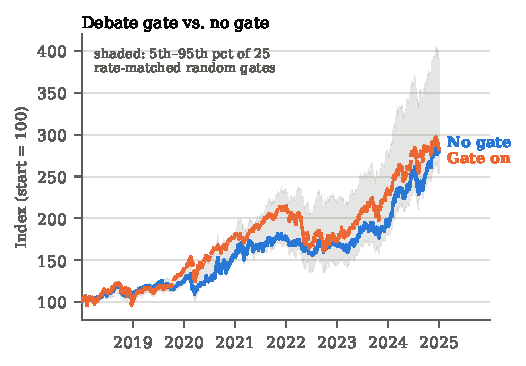
\includegraphics[width=\columnwidth]{fig_gate.pdf}
\caption{The debate-gate experiment. Both arms consume an identical signal
stream; the gated arm executes only what the panel approved. The shaded band is
the 5th--95th percentile of 25 gates that reject at the same rate but choose at
random. The gated arm spends the entire window inside that band and ends inside
it, which is the finding: whatever the panel contributed is within the range of
rejecting the same number of trades arbitrarily.}
\label{fig:gate}
\end{figure}

\textbf{The control that decides the question.} A gate rejecting 59.6\% of
trades changes exposure and turnover whether or not it chooses well, and on
this sample those mechanical effects are large. Arm~C therefore rejects at
the same 59.6\% rate but picks at random. Twenty-five such gates returned a
Sharpe of 0.93 $\pm$ 0.14 (5th--95th percentile 0.73--1.19), and the LLM
panel beat only 5 of them, an empirical $p$ of 0.80.

Fig.~\ref{fig:gate} describes why that comparison, rather than the A-versus-B
one, settles the question. It plots the equity curve of the gated arm against a
shaded band spanning the 5th--95th percentile of the 25 random gates, so the
band is the range of outcomes available from rejecting 59.6\% of trades with no
judgment at all. The gated curve enters that band immediately, stays inside it
for the whole seven years, and ends inside it: at no point does the panel's
selection separate from arbitrary rejection at the same rate. Random rejection
was in fact better than the panel, on average and at the median. The
parsimonious reading is that the gate's effect here is the effect of trading
less, and the deliberation added nothing on top of it. Without this control the
turnover reduction would have been written up as a risk-management benefit.

\textbf{Was the panel simply remembering?} On 44 signals judged both ways, the
unblinded panel approved 34.1\% against the blinded panel's 38.6\% and reached
the same verdict on 73\% of individual trades (Table~\ref{tab:leak}). Mean
consensus scores were 0.384 and 0.374. Revealing the ticker and the date
barely moved anything, which is the result the blinded design needs: the panel
was working from the features it was given, not recalling what the stock did
next. The paired sample is small, and the claim goes no further than that.

\textbf{A note on the counterfactual.} Summed over the 161 rejections with
price coverage, the trades the gate blocked would have returned $-101\%$ of
NAV, and only 38\% of them would have made money. Read naively that says the
vetoes were good, which sits awkwardly beside an arm that performed worse. The
two are not in conflict, but the counterfactual is the weaker number. It adds
up each blocked weight change multiplied by its own forward return, treating
the rejections as independent one-at-a-time events. The arm they belong to
compounds, overlaps and rebalances, and it carries the cost of the stale
positions the vetoes left in place, which the sum does not see. The figure
is reported because it was pre-registered; where it and the arm-level result
point in different directions, the arm-level result and Arm~C carry the weight.

Under the criterion fixed in Sec.~\ref{sec:aitest} (arm~B's risk-adjusted
return at least equal to arm~A's \emph{and} non-positive counterfactual P\&L),
the gate \textbf{fails} on the first condition and reverts to
advisory-only. The debate layer keeps its other job. Every trade still carries
a recorded argument for why it was permitted, and in a system that trades
without a human in the loop that record has value independent of whether the
votes improve returns. It has not earned authority over execution.

\subsection{What the Result Says About the Architecture}

It is worth separating two claims that are easy to run together. The debate
gate did not improve returns. The \emph{system} was unaffected by that: it
continued to trade, to size against a database-backed ledger, to enforce its
risk limits, and to route orders correctly, because the gate sits in a veto
slot where its failure mode is a trade that does not happen. Arm~B's worst
outcome across seven years was a Sharpe ratio 0.08 below arm~A's. It was not a
blown risk limit, an unbounded position, or a ledger that stopped reconciling.

That is the property the three-gate structure was built for, and it is the one
that matters for a system intended to run without supervision. A design in
which the least predictable component is load-bearing converts a model failure
into a capital loss, which is the failure mode that machine-learning systems
accumulate quietly as their components grow entangled \cite{sculley2015debt}.
Here the least predictable component is advisory by construction, its authority
is a veto rather than an instruction, and removing it entirely returns the
system to a configuration that has already been measured. Reporting that an LLM
layer added nothing is preferable to reporting that it worked until it did not.

The practical consequence is a deployment posture rather than a deletion. The
gate ships enabled in its advisory role, where it produces the audit trail, and
disabled as a binding veto until it can clear the control in
Sec.~\ref{sec:aitest} under conditions the architecture was designed for and
this run could not supply: more than one model family, and a sentiment role
with a point-in-time news archive to reason from.

\begin{table}[t]
\caption{Debate-gate A/B, blinded panel, PIT 2018--2024. Identical signal
stream and fill model across arms. Arm~C holds arm~B's rejection rate but
chooses at random (25 trials, mean $\pm$ s.d.).}
\label{tab:abtest}
\centering
\setlength{\tabcolsep}{4pt}
\footnotesize
\begin{tabular}{lccc}
\toprule
Metric & A (no gate) & B (gate on) & C (random) \\
\midrule
Trades executed & 1{,}867 & 1{,}510 & 1{,}722 \\
Rejection rate & n/a & 59.6\% & 59.6\% \\
Counterfactual P\&L$^\ddagger$ & n/a & $-101\%$ & n/a \\
CAGR & 15.9\% & 15.9\% & n/a \\
Volatility & 15.3\% & 17.3\% & n/a \\
Sharpe ratio & \textbf{0.89} & 0.81 & 0.93 $\pm$ 0.14 \\
Sortino ratio & \textbf{1.16} & 1.05 & n/a \\
Max drawdown & $\mathbf{-18.0\%}$ & $-25.7\%$ & n/a \\
Turnover ($\times$ NAV/yr) & 12.72 & 2.69 & n/a \\
\bottomrule
\end{tabular}

\vspace{2pt}
{\footnotesize $^\ddagger$A sum of independent one-at-a-time effects, not a
realizable P\&L; see the discussion in Sec.~\ref{sec:abresults}. Arm~C executes
more trades than arm~B at the same rejection rate because it rejects a
different, randomly chosen subset.}
\end{table}

\begin{table}[t]
\caption{Hindsight-leakage sensitivity: the same signals judged with the
security's identity and date withheld (primary) and restored (sensitivity).
A large gap would indicate the panel is recalling outcomes rather than
reasoning from features.}
\label{tab:leak}
\centering
\begin{tabular}{lcc}
\toprule
Metric & Blinded & Unblinded \\
\midrule
% BEGIN:leak-rows
Debates (paired) & 44 & 44 \\
Approval rate & 38.6\% & 34.1\% \\
Verdict agreement with blinded & n/a & 72.7\% \\
Mean consensus score & 0.384 & 0.374 \\
% END:leak-rows
\bottomrule
\end{tabular}
\end{table}

\section{Limitations}
\label{sec:limits}

\textbf{No real capital.} Everything here is a backtest on daily bars plus a
live \emph{paper}-trading deployment (Sec.~\ref{sec:live}).

\textbf{The peer comparison is tilted in this system's favour.} The hedge-fund
and balanced benchmarks are realized, investable, net-of-fee return streams
carrying management costs and capacity constraints. The strategy rows charge
commissions and market impact but no management or performance fee, and assume
the strategy's own capacity is unbounded. The peer rows should be read as an
indication that the mix is in a competitive range, not as evidence of realized
excess return over the industry.

\textbf{Residual survivorship bias.} Free daily data omits many delisted
securities \cite{shumway1997delisting}: 85\% of the point-in-time union was
recovered on 2018--2024 and 71\% on 2008--2017, where the shortfall is
concentrated in crisis-era delistings. Every arm and benchmark is affected
identically, so the ordering should hold, but absolute return levels are
optimistic by an amount that cannot be measured without a paid
survivorship-free vendor.

\textbf{One historical path.} A Sharpe ratio estimated from a single
realization overstates certainty \cite{bailey2014deflated,lo2002statistics}.
Sec.~\ref{sec:dsr} deflates for the variants tried, which narrows the problem
without removing it. The prediction-market study is weaker still: few markets,
short window.

\textbf{The debate-gate experiment.} Four limitations attach to it
specifically. First, it is a \emph{replay}: the panel judges
historical signals rather than trading forward, which buys the sample size the
pre-registered metrics need at the cost of the leakage risk quantified in
Table~\ref{tab:leak}. Blinding removes the security's identity and date, but
an extreme feature combination can still narrow the era, so the residual is
bounded rather than zero. Second, the panel ran on a \emph{single} provider.
The architecture assigns roles across model families and the mechanism is
exercised in live operation, but the reported experiment does not demonstrate
cross-family diversity, and same-family debaters may share failure modes that
independent families would not. Third, the \textsc{sentiment} role abstains
structurally in replay: no point-in-time news archive is available, and the
role is instructed to abstain rather than guess, so roughly one voice in four
contributes little to the reported verdicts. Fourth, the gate was evaluated in
its \emph{deployed} configuration, judging the strongest signals within a
budget rather than every signal; the effect of gating the full stream is
unmeasured and would require an order of magnitude more model calls.

\textbf{LLM judgments inherit the biases of their training corpora}, and for a
closed model there is no way to audit what those are. This bounds the blinding
argument: the panel demonstrably behaved almost identically with and without
the ticker, which rules out one specific failure, but says nothing about
whether its priors on momentum or volatility are calibrated to the period it
was judging.

\section{Toward Production}
\label{sec:production}

This is not a deployable fund. The claim is narrower: the distance between this
system and one is measurable, and most of what remains is capital and time
rather than unsolved design. This section separates the two.

\textbf{What has been demonstrated.} The pipeline has traded end to end against
a real brokerage API: sleeve signals became live orders, orders were polled to
terminal fills including fractional shares, and cash settled atomically exactly
once per order, a property the accounting tests pin, because a
settle-twice bug is invisible until the ledger diverges. The system runs on a
laptop with no external services, so operating it does not presuppose
infrastructure. It survives its own faults: a supervisor restarted four agents
that crashed on a boot-time database contention without operator action, and
the reconciliation guard of Sec.~\ref{sec:live} caught a $3.5\times$ leverage
exposure created by a ledger that disagreed with the broker. Risk limits, the
kill switch and the naked-short prohibition are enforced in the execution path
rather than advised, and 467 automated tests hold the validated mix weights and
the cash/P\&L identity in place against regression.

\textbf{What is missing, in the order it would have to be fixed.} First, real
capital, in an amount small enough that the loss is tuition, under the same
gates and with the same reconciliation guard active. Nothing in this paper
substitutes for that, and a live track record is the only evidence that settles
the questions a backtest cannot: fill quality at size, borrow availability,
and whether the operator actually leaves the system alone. Second, capacity.
The fill model charges commission and impact but assumes the strategy's own
participation does not move the book; the top-five concentration of the
research sleeve makes that assumption fail sooner than it would for a
diversified mandate. Third, the
sentiment role needs a point-in-time news archive before it contributes
anything; at present it abstains, and one silent voice in four is a design
that is not being tested. Fourth, the debate gate needs the multi-family
configuration it was written for. Fifth, and least technical: anyone operating
this on behalf of other people inherits a regulatory perimeter that this paper
does not address at all.

\textbf{What to tell someone considering building on it.} The parts worth
trusting are the ones that were tested adversarially and the ones that have
already failed once and been fixed: the reconciliation guard, the settlement
path, the risk gates, and the validation protocol itself. The part not yet
worth trusting with authority is the part that is most fashionable. That
ordering is the opposite of how such systems are usually presented, and it is
the honest one.

\section{Conclusion}

Horizon Capital works. A firm of decoupled agents, three nested gates between a
signal and a broker order, running on a laptop against a real brokerage API,
producing a book that would have turned \$100{,}000 into \$340{,}322 across the
financial crisis while the index reached \$226{,}948 and lost half its value on
the way. The part worth defending in a seminar, though, is not the return. It
is the protocol that decided what got to stay in the system.

That protocol took away more than it gave, which is the point. It took away the
edge that started the project, once point-in-time membership showed it was
survivorship bias. It took away a breadth sleeve carrying 40\% of the mix,
after leave-one-out attribution showed the ensemble was better without it. It
rejected a top-10 momentum variant and a prediction-market sleeve. What
survived is regime-gated momentum and quality with trend and momentum-rank
satellites at 0.500/0.333/0.167, and it returns a Sharpe of 0.89 and 0.99 on
the two windows against 0.64 and 0.49 for the index, at lower volatility, with
roughly half the drawdown, and with a deflated probability of a positive true
Sharpe of 0.72 and 0.85 after accounting for the twelve variants tried.

The same protocol then took away the component the project had been most
confident in. Under blinded prompts and a control that rejected trades at the
same rate but chose at random, the LLM debate gate did not beat the control,
and the improvement that would otherwise have been claimed turned out to be a
fivefold reduction in turnover wearing a different hat. That control belongs in
any study of an LLM gate, filter or veto, precisely because such mechanisms
change trading behaviour in ways that move performance on their own. This one
would have looked like a modest success without it.

None of this says LLMs cannot contribute to a trading system. It says this
gate, in this configuration, on these signals, did not, and that the only
reason this is known is that it was checked. The next steps follow from the
limitations: run the panel across genuinely different model families rather
than one, supply a point-in-time news archive so the sentiment role has
something to reason about instead of abstaining, test the gate on the full
signal stream rather than the strongest 58\% of traded weight, and extend the
same point-in-time treatment to the crypto sleeve before any of it sees real
capital.

\begin{thebibliography}{35}

\bibitem{yang2020ensemble}
H.~Yang, X.-Y.~Liu, S.~Zhong, and A.~Walid, ``Deep reinforcement learning
for automated stock trading: An ensemble strategy,'' in \emph{Proc. ACM
Int. Conf. AI in Finance (ICAIF)}, 2020.

\bibitem{xiong2018practical}
Z.~Xiong, X.-Y.~Liu, S.~Zhong, H.~Yang, and A.~Elwalid, ``Practical deep
reinforcement learning approach for stock trading,'' \emph{NeurIPS Workshop
on Challenges and Opportunities for AI in Financial Services}, 2018.

\bibitem{jiang2017deep}
Z.~Jiang, D.~Xu, and J.~Liang, ``A deep reinforcement learning framework for
the financial portfolio management problem,'' \emph{arXiv:1706.10059}, 2017.

\bibitem{liu2020finrl}
X.-Y.~Liu, H.~Yang, Q.~Chen, R.~Zhang, L.~Yang, B.~Xiao, and C.~D.~Wang,
``FinRL: A deep reinforcement learning library for automated stock trading in
quantitative finance,'' \emph{Deep RL Workshop, NeurIPS}, 2020.
\emph{arXiv:2011.09607}.

\bibitem{kim2025mama}
S.-H.~Kim and K.-H.~Lee, ``Multi-asset multi-agent reinforcement learning for
portfolio management,'' \emph{IEEE Access}, vol.~13, 2025,
doi:10.1109/ACCESS.2025.3632201.

\bibitem{park2024uncertainty}
K.~Park, H.-G.~Jung, T.-S.~Eom, and S.-W.~Lee, ``Uncertainty-aware portfolio
management with risk-sensitive multiagent network,'' \emph{IEEE Trans. Neural
Networks and Learning Systems}, vol.~35, no.~1, 2024.

\bibitem{sun2024graphsage}
Q.~Sun, X.~Wei, and X.~Yang, ``GraphSAGE with deep reinforcement learning for
financial portfolio optimization,'' \emph{Expert Systems with Applications},
vol.~238, art.~122027, 2024.

\bibitem{sun2024dynamic}
H.~Sun, Y.~Bian, L.~Han, P.~Zhu, D.~Cheng, and Y.~Liang, ``Dynamic graph-based
deep reinforcement learning with long and short-term relation modeling for
portfolio optimization,'' in \emph{Proc. 33rd ACM Int. Conf. Information and
Knowledge Management (CIKM)}, 2024.

\bibitem{liu2025qtmrl}
X.~Liu and J.~Chen, ``QTMRL: An agent for quantitative trading decision-making
based on multi-indicator guided reinforcement learning,''
\emph{arXiv:2508.20467}, 2025.

\bibitem{yang2023fingpt}
H.~Yang, X.-Y.~Liu, and C.~D.~Wang, ``FinGPT: Open-source financial large
language models,'' \emph{arXiv:2306.06031}, 2023.

\bibitem{wu2023bloomberggpt}
S.~Wu \emph{et al.}, ``BloombergGPT: A large language model for finance,''
\emph{arXiv:2303.17564}, 2023.

\bibitem{du2023improving}
Y.~Du, S.~Li, A.~Torralba, J.~B.~Tenenbaum, and I.~Mordatch, ``Improving
factuality and reasoning in language models through multiagent debate,''
\emph{arXiv:2305.14325}, 2023.

\bibitem{park2023generative}
J.~S.~Park, J.~O'Brien, C.~J.~Cai, M.~R.~Morris, P.~Liang, and
M.~S.~Bernstein, ``Generative agents: Interactive simulacra of human
behavior,'' in \emph{Proc. ACM UIST}, 2023.

\bibitem{xiao2024tradingagents}
Y.~Xiao, E.~Sun, D.~Luo, and W.~Wang, ``TradingAgents: Multi-agents LLM
financial trading framework,'' \emph{arXiv:2412.20138}, 2024.

\bibitem{yu2023finmem}
Y.~Yu, H.~Li, Z.~Chen, Y.~Jiang, Y.~Li, D.~Zhang, R.~Liu, J.~W.~Suchow, and
K.~Khashanah, ``FinMem: A performance-enhanced LLM trading agent with layered
memory and character design,'' \emph{arXiv:2311.13743}, 2023.

\bibitem{li2025quantagents}
X.~Li, Y.~Zeng, X.~Xing, J.~Xu, and X.~Xu, ``QuantAgents: Towards multi-agent
financial system via simulated trading,'' \emph{arXiv:2510.04643}, 2025.

\bibitem{glasserman2023lookahead}
P.~Glasserman and C.~Lin, ``Assessing look-ahead bias in stock return
predictions generated by GPT sentiment analysis,'' \emph{arXiv:2309.17322},
2023.

\bibitem{palomo2023tweet}
C.~Palomo, ``Tweet sentiment analysis to predict stock market,'' Stanford
CS224N custom project report, 2023.

\bibitem{ma2025hedge}
T.~Ma, W.~Wang, and F.~Jiang, ``Machine learning the performance of hedge
funds,'' \emph{Journal of International Money and Finance}, vol.~155,
art.~103332, 2025.

\bibitem{cerneviciene2024xai}
J.~\v{C}ernevi\v{c}ien\.{e} and A.~Kaba\v{s}inskas, ``Explainable artificial
intelligence (XAI) in finance: A systematic literature review,''
\emph{Artificial Intelligence Review}, vol.~57, art.~216, 2024.

\bibitem{bartram2020ai}
S.~M.~Bartram, J.~Branke, and M.~Motahari, \emph{Artificial Intelligence in
Asset Management}. CFA Institute Research Foundation Literature Review, 2020.

\bibitem{wang2015concept}
H.~Wang and Z.~Abraham, ``Concept drift detection for streaming data,'' in
\emph{Proc. Int. Joint Conf. Neural Networks (IJCNN)}, 2015.

\bibitem{sculley2015debt}
D.~Sculley \emph{et al.}, ``Hidden technical debt in machine learning
systems,'' in \emph{Advances in Neural Information Processing Systems
(NeurIPS)}, 2015.

\bibitem{eugster2003faces}
P.~T.~Eugster, P.~A.~Felber, R.~Guerraoui, and A.-M.~Kermarrec, ``The many
faces of publish/subscribe,'' \emph{ACM Computing Surveys}, vol.~35, no.~2,
pp. 114--131, 2003.

\bibitem{jegadeesh1993returns}
N.~Jegadeesh and S.~Titman, ``Returns to buying winners and selling losers:
Implications for stock market efficiency,'' \emph{Journal of Finance},
vol.~48, no.~1, pp. 65--91, 1993.

\bibitem{faber2007tactical}
M.~T.~Faber, ``A quantitative approach to tactical asset allocation,''
\emph{Journal of Wealth Management}, vol.~9, no.~4, pp. 69--79, 2007.

\bibitem{asness2019qmj}
C.~S.~Asness, A.~Frazzini, and L.~H.~Pedersen, ``Quality minus junk,''
\emph{Review of Accounting Studies}, vol.~24, pp. 34--112, 2019.

\bibitem{lopezdeprado2016hrp}
M.~L\'opez~de~Prado, ``Building diversified portfolios that outperform
out of sample,'' \emph{Journal of Portfolio Management}, vol.~42, no.~4,
pp. 59--69, 2016.

\bibitem{kelly1956}
J.~L.~Kelly, ``A new interpretation of information rate,'' \emph{Bell
System Technical Journal}, vol.~35, no.~4, pp. 917--926, 1956.

\bibitem{maclean2011kelly}
L.~C.~MacLean, E.~O.~Thorp, and W.~T.~Ziemba, Eds., \emph{The Kelly Capital
Growth Investment Criterion: Theory and Practice}. World Scientific, 2011.

\bibitem{moskowitz2012tsmom}
T.~J.~Moskowitz, Y.~H.~Ooi, and L.~H.~Pedersen, ``Time series momentum,''
\emph{Journal of Financial Economics}, vol.~104, no.~2, pp. 228--250, 2012.

\bibitem{hamilton1989regime}
J.~D.~Hamilton, ``A new approach to the economic analysis of nonstationary
time series and the business cycle,'' \emph{Econometrica}, vol.~57, no.~2,
pp. 357--384, 1989.

\bibitem{bailey2014deflated}
D.~H.~Bailey and M.~L\'opez~de~Prado, ``The deflated Sharpe ratio:
Correcting for selection bias, backtest overfitting and non-normality,''
\emph{Journal of Portfolio Management}, vol.~40, no.~5, pp. 94--107, 2014.

\bibitem{lopezdeprado2018advances}
M.~L\'opez~de~Prado, \emph{Advances in Financial Machine Learning}.
Wiley, 2018.

\bibitem{kritzman2012regime}
M.~Kritzman, S.~Page, and D.~Turkington, ``Regime shifts: Implications for
dynamic strategies,'' \emph{Financial Analysts Journal}, vol.~68, no.~3,
pp. 22--39, 2012.

\bibitem{almgren2001optimal}
R.~Almgren and N.~Chriss, ``Optimal execution of portfolio transactions,''
\emph{Journal of Risk}, vol.~3, no.~2, pp. 5--39, 2001.

\bibitem{markowitz1952}
H.~Markowitz, ``Portfolio selection,'' \emph{Journal of Finance}, vol.~7,
no.~1, pp. 77--91, 1952.

\bibitem{sharpe1994}
W.~F.~Sharpe, ``The Sharpe ratio,'' \emph{Journal of Portfolio Management},
vol.~21, no.~1, pp. 49--58, 1994.

\bibitem{sortino1994downside}
F.~A.~Sortino and L.~N.~Price, ``Performance measurement in a downside risk
framework,'' \emph{Journal of Investing}, vol.~3, no.~3, pp. 59--64, 1994.

\bibitem{young1991calmar}
T.~W.~Young, ``Calmar ratio: A smoother tool,'' \emph{Futures}, vol.~20,
no.~1, 1991.

\bibitem{lo2002statistics}
A.~W.~Lo, ``The statistics of Sharpe ratios,'' \emph{Financial Analysts
Journal}, vol.~58, no.~4, pp. 36--52, 2002.

\bibitem{bailey2012psr}
D.~H.~Bailey and M.~L\'opez~de~Prado, ``The Sharpe ratio efficient frontier,''
\emph{Journal of Risk}, vol.~15, no.~2, pp. 3--44, 2012.

\bibitem{harvey2016cross}
C.~R.~Harvey, Y.~Liu, and H.~Zhu, ``$\ldots$ and the cross-section of expected
returns,'' \emph{Review of Financial Studies}, vol.~29, no.~1, pp. 5--68,
2016.

\bibitem{elton1996survivorship}
E.~J.~Elton, M.~J.~Gruber, and C.~R.~Blake, ``Survivorship bias and mutual
fund performance,'' \emph{Review of Financial Studies}, vol.~9, no.~4,
pp. 1097--1120, 1996.

\bibitem{shumway1997delisting}
T.~Shumway, ``The delisting bias in CRSP data,'' \emph{Journal of Finance},
vol.~52, no.~1, pp. 327--340, 1997.

\bibitem{fung2000performance}
W.~Fung and D.~A.~Hsieh, ``Performance characteristics of hedge funds and
commodity funds: Natural vs. spurious biases,'' \emph{Journal of Financial and
Quantitative Analysis}, vol.~35, no.~3, pp. 291--307, 2000.

\bibitem{wolfers2004prediction}
J.~Wolfers and E.~Zitzewitz, ``Prediction markets,'' \emph{Journal of Economic
Perspectives}, vol.~18, no.~2, pp. 107--126, 2004.

\bibitem{kirilenko2017flash}
A.~Kirilenko, A.~S.~Kyle, M.~Samadi, and T.~Tuzun, ``The flash crash:
High-frequency trading in an electronic market,'' \emph{Journal of Finance},
vol.~72, no.~3, pp. 967--998, 2017.

\bibitem{sec2013knight}
U.S. Securities and Exchange Commission, ``In the matter of Knight Capital
Americas LLC,'' Administrative Proceeding File No.~3-15570, Release
No.~34-70694, Oct. 2013.

\end{thebibliography}

\end{document}
